
\section{Essence of Semantic Model Adaptation}
\label{ch:essence_of_adaptation}

% 因為有很多Model, 卻有更多問題, 我們懷疑
%懷疑 假說 實驗



This chapter shows the essence of semantic model adaptation. Due to the different semantics of permutation problems, it is non-trivial to determine which model. Besides, the semantics of some permutation problem needs more than one model to describe. PFSP is an example of such problem that needs models which can handle connection of nodes and absolution position of nodes~\citep{tsutsui2006node}. 

The semantics go beyond the capability of existing models. As a result, existing models can not capture the semantics precisely. For example, LOP, of which objective function is mainly contributed by the order of indices, can not be interpreted precisely by either NHM or EHM. When it comes the real-world problems, the semantics in the permutation may even complicated~\citep{ceberio2012review}. For this reason, the capability of solving the more complicated permutation problems is crucial.

\subsection{Effects of Different Models}
As a semantic model can only express specific permutation problems, model-choosing becomes critical. For illustration, the following experiment uses TSP and QAP as example. In TSP, the relative ordering of each indices in permutations contributes the fitness. However, the information drawn from the absolute positions of each indices are useless. In contrast, on QAP, the quality of the solution is determined by the absolute position of each index in the permutation. Hence, the relative ordering of the indices in permutation does not matter for QAP.


  For investigating the capability of different semantic models, we test EHBSA and EHBSA on QAP and TSP with the population size $N = 2 \times L$ and the NFE limit $E_{max} = L \times 40000$ , where $L$ is the problem size. For every instance, we perform 10 independent runs.

 The experiment settings are as follows: 
\begin{itemize}
   % \item repeating 10 times,
   % \item performing NHBSA and EHBSA on QAP and TSP, template technique is used,
   % \item population size $N = 2 \times L$ ($L$ is the problem size),
   % \item the bias ratio $B_{ratio} = 0.0000$,
   % \item the NFE $E_{max} = L \times 40000$ and
   % \item the cut-point number is 3 for template.
\end{itemize}

\begin{table}[t]
    \centering
    \begin{subtable}{.45\linewidth}\centering
        \begin{tabular}{|l|l|l|}
        \hline
                           & \textbf{NHBSA} & \textbf{EHBSA} \\ \hline
        \textbf{bayg29}    & $1.34\times 10^{-1}$       & $0.00$       \\ \hline
        \textbf{dantzig42} & $4.69\times 10^{-1}$       & $1.43\times 10^{-3}$       \\ \hline
        \textbf{eil51}     & $5.59\times 10^{-1}$       & $0.00$       \\ \hline
        \textbf{berlin52}  & $5.55\times 10^{-1}$       & $0.00$       \\ \hline
        \textbf{eil76}     & $9.72\times 10^{-1}$       & $1.86\times 10^{-4}$      \\ \hline
        \end{tabular}
        \caption{TSP}
        \label{tb:TSP}
    \end{subtable}
    \hfill{}
    \begin{subtable}{.45\linewidth}\centering
        \begin{tabular}{|l|l|l|}
        \hline
                        & \textbf{NHBSA} & \textbf{EHBSA} \\ \hline
        \textbf{nug18}  & $3.11\times 10^{-4}$       & $8.50\times 10^{-3}$       \\ \hline
        \textbf{nug17}  & $0.00$       & $1.15\times 10^{-3}$       \\ \hline
        \textbf{nug21}  & $6.56\times 10^{-4}$       & $1.05\times 10^{-2}$       \\ \hline
        \textbf{bur26b} & $1.82\times 10^{-4}$       & $1.36\times 10^{-3}$       \\ \hline
        \textbf{bur26a} & $2.58\times 10^{-4}$       & $1.51\times 10^{-3}$       \\ \hline
        \end{tabular}
        \caption{QAP}
        \label{QAP}
    %\hfill{}
    \end{subtable}
\caption{Average error for each instance}
\label{tb:model_choosing}
\end{table}

Table \ref{tb:model_choosing} shows the average error for each instance of problems. The average error is calculated as the normalized difference between the best objective value obtained by the algorithm and the best known solution. The lower the values are, the better the performance. As can been seen, the EHBSA outperforms the NHBSA in all instances of TSP. In contrast, the NHBSA outperforms the EHBSA in all instances of QAP. 

This result confirms that model-choosing is crucial for EDAs for permutation problems. This performance difference between these two models starts from the design. In other word, EHM captures the adjacency of indices which matches the semantics of TSP, while NHM captures the absolute positions of indices which is more fitted on QAP. These differences makes the nature that before solving any permutation problem, a semantic model which is able to describe the semantics of the problem should be chosen.

Although model-choosing significantly affects the performance, the semantics of permutation problem is not always so clear for the literature~\citep{ceberio2012review}. For instance, the objective function of the permutation flow-shop scheduling problem (PFSP) is given by the completion time of the last job that depends on the ordering of the jobs. Intuitively, EHM is the best choice for PFSP, but the empirical result shows that NHM ties with EHM. For this reason, model-choosing rises the difficulty for solving permutation problems.



\subsection{Verification by sweeping}

%\begin{figure}[t]
%    \begin{algorithm}[H]
%        \For{$p=0.0;\, p \leq 1.0;\, p = p + 0.1$}{
%            hybrid algorithm with EHM($p$), NHM($1-p$)\;
%            record the best solution of this trial\;
%        }
%        \caption{The Sweep Method}
%        \label{alg:sweep_method}
%    \end{algorithm}
%    \begin{algorithm}[H]
%        generate initial population $P$\;
%        \While{not meet the terminate criterion}{
%            select population of promising solution $S$\;
%            build probabilistic model $M$ for $S$\;
%            sample $M$ to generate offspring set $O$\;
%            incorporate $O$ into $P$\;
%        }
%        \caption{The Hybrid Algorithm}
%        \label{alg:hybrid_algorithm}
%    \end{algorithm}
%\end{figure}

Since some problems exist, of which the semantics is not exactly belong the index adjacency or absolute position, incorporating different models is a way to achieve higher fitness. In order to investigate the potential for improvement, we hybridizes EHM and NHM in the model-building stage in EDAs. 

In our experiments,we performs a trial of hybridization of EHM and NHM. The hybrid algorithm generally follows Tsutsui's evolutionary model, but with some modification. Different from Tsutsui's evolutionary model~\citep{tsutsui2006comparative}, the hybrid algorithm picks one model to sample new individuals with the given probability and updates both models at the same time. The probability for the EHM $p$ starts from $0.0$ to $1.0$ and increases $0.1$ by each iteration. Then, we perform the hybrid algorithm with the population size $N = 2 \times L$ and the NFE limit $E_{max} = L \times 40000$ independent 10 runs on each iteration. After each trial, we records its the best solution and its objective function value. LOP and PFSP are tested in our experiments, and four instances of each problem are picked: $t65b11x$,  $t65d11x$, $t65f11x$ and $t65n11x$ from LOLIB\footnote{http://www.optsicom.es/lolib/} and  $ta021$, $ta041$, $ta051$ and $ta071$ from Taillard's instance library \footnote{http://mistic.heig-vd.ch/taillard/problemes.dir/ordonnancement.dir/ordonnancement.html}. In the end, the best mixing ratio of models is revealed. 



% \begin{figure}[t]
    % \centering
    % \begin{subfigure}{1.0\textwidth}
        % 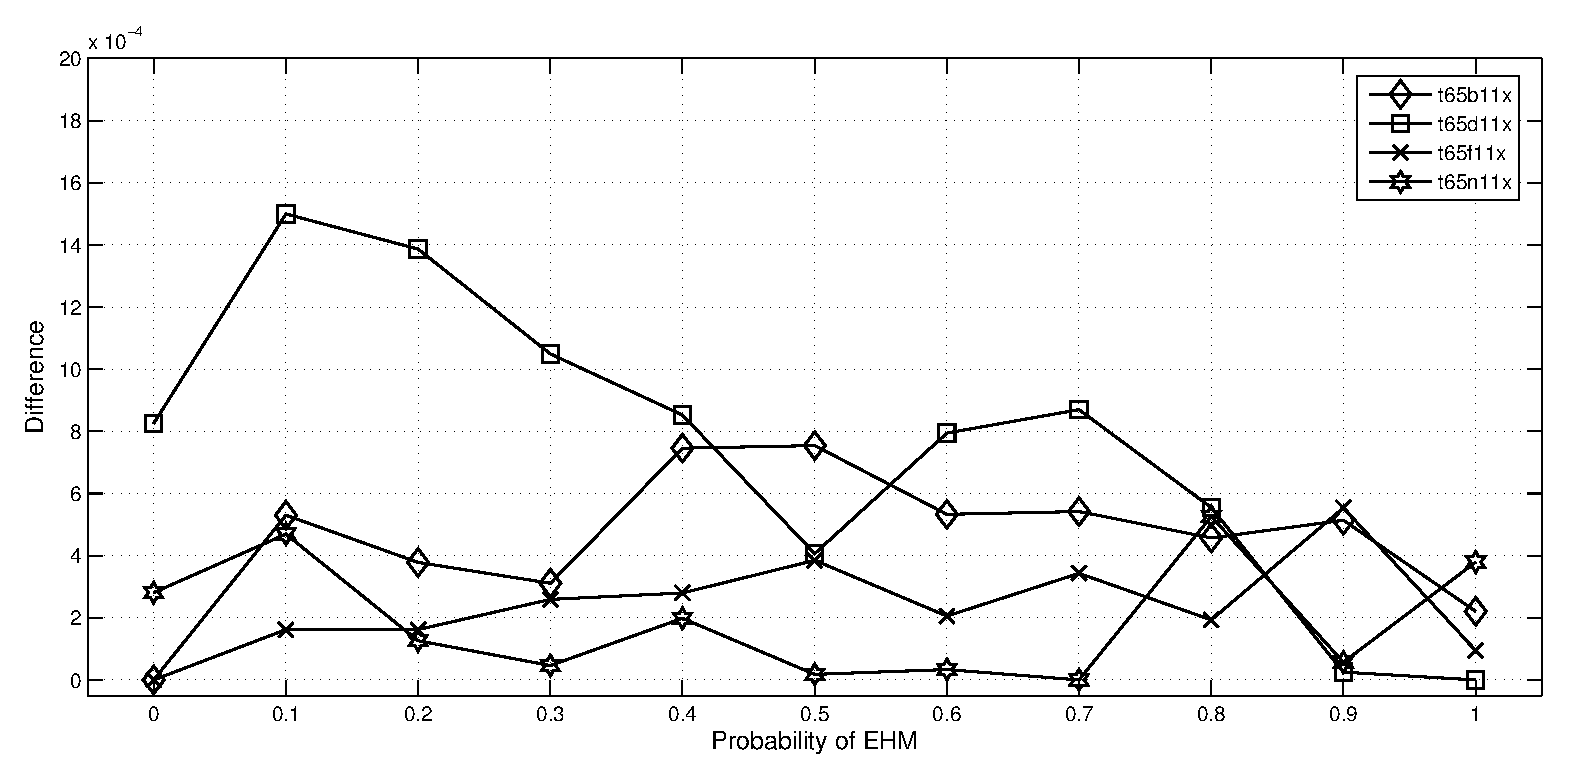
\includegraphics[width=1.0\textwidth]{img/sweep_lop.eps}
        % \caption{LOP}
    % \end{subfigure}\\
    % \begin{subfigure}{1.0\textwidth}
        % 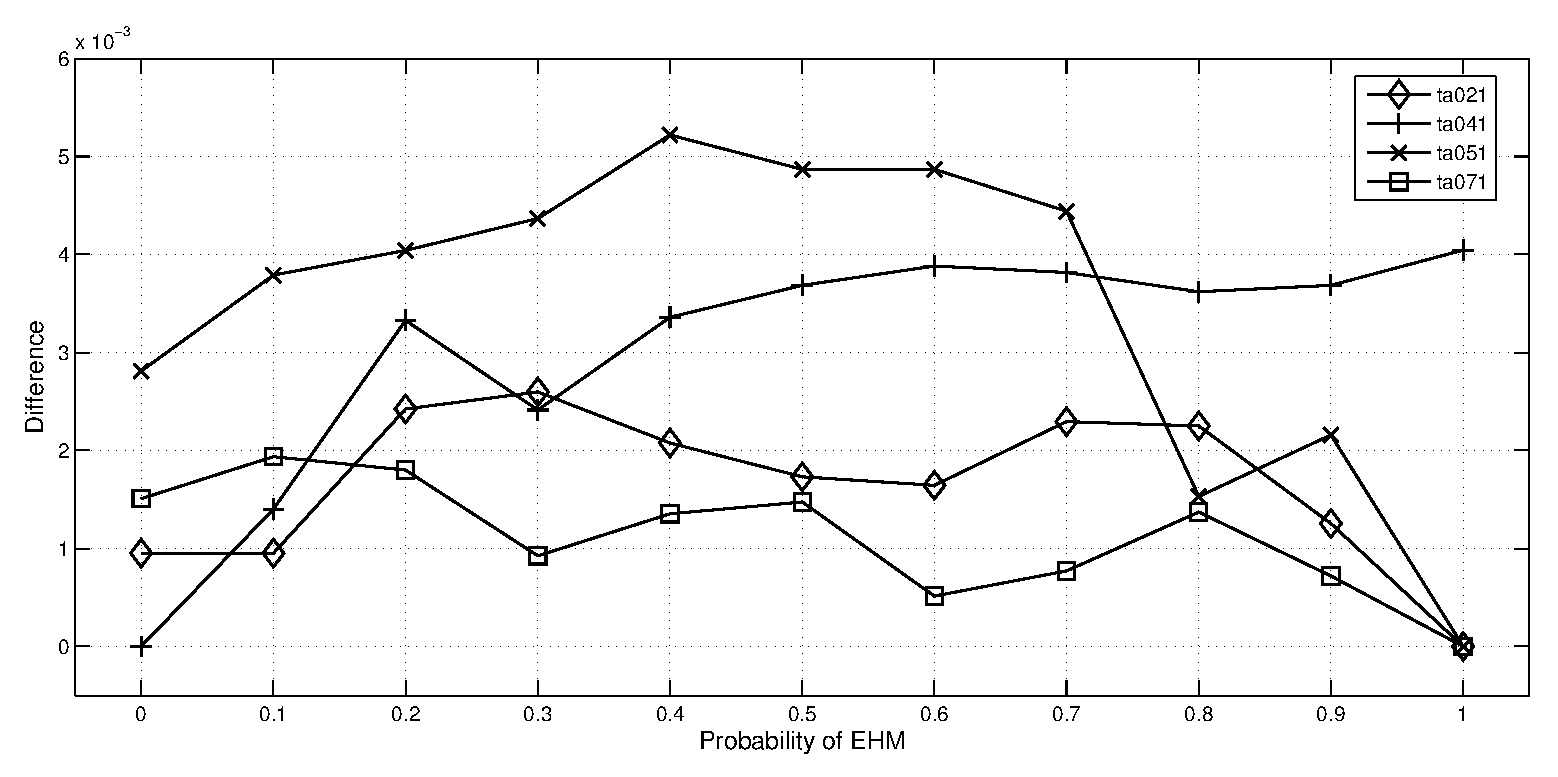
\includegraphics[width=1.0\textwidth]{img/sweep_pfsp.eps}
        % \caption{PFSP}
    % \end{subfigure}
    % \caption{Difference of average of each probability $p$ }
    % \label{fig:sweep}
% \end{figure}

\begin{figure}[t]
    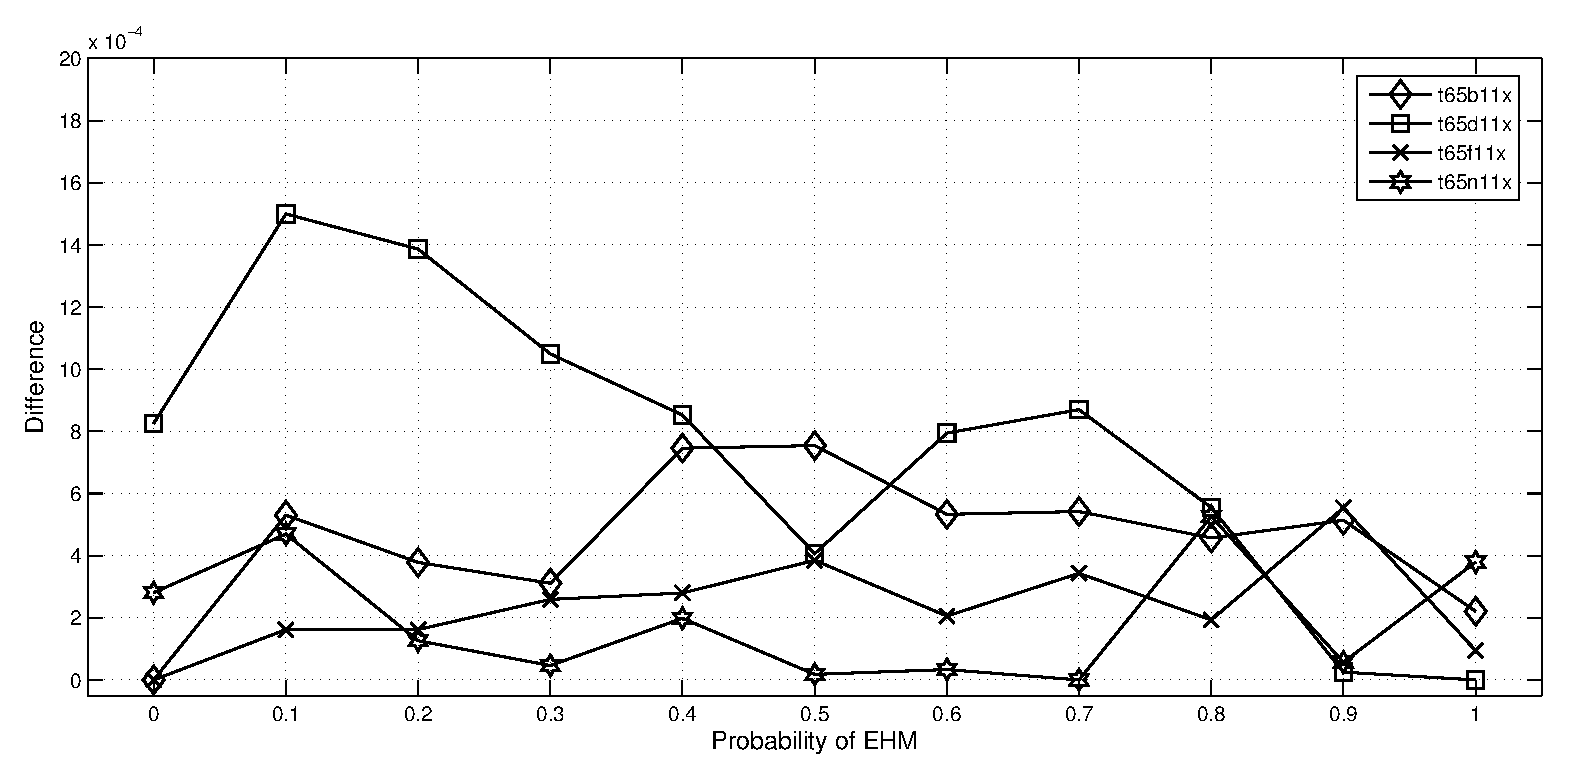
\includegraphics[width=1.0\textwidth]{img/sweep_lop.eps}

    \caption{Difference of average of each probability $p$ on LOP}
    \label{fig:sweep_lop}
\end{figure}









Figures \ref{fig:sweep_lop} shows the difference between average of each probability. The values on the $y$-axis is the normalized difference between the average the best objective values in each trial and the worst average of object values among all trials. The higher the values is, the better the performance. The values on the $x$-axis are the probability $p$ of to sampling EHM. In other word, the value $p=1.0$ indicates that the hybrid algorithm is identical to EHBSA which is by pure EHM, and the value $p=0.0$ indicates that the hybrid algorithm is identical to NHBSA which is by pure NHM.

As can be seen, in some instances of PFSP, the best objective value is obtained in the trials that both models have chance to sample new individual. In all of the instances of LOP, the experiments with only one model have lower object value than the one with hybridization of two models. These experiments indicate that mixing different models can be more efficient when solving permutation problems. Thus, we make the three attempt at model adaptation in the follow chapters.


% \subsection{Summary}
% In this chapter, the model-choosing experiment shows the impact of inappropriate model. Since the model-choosing significantly effects the performance of the EDAs for permutation problem, the semantics of problems must be studied for better performance. But the semantics of real-life problems is not always trivial as TSP and QAP. It makes finding a appropriate model a difficult task. Next, the second experiment uses the sweep method to investigate the improvement possibility of incorporating multi-models. The result shows that incorporating multi-models can achieve better performance on problems like PFSP and LOP which models cannot precisely describe.
